\chapter{Especificação e Modelação}

\section{Análise de Requisitos}

\subsection{Requisitos Funcionais}

\subsubsection{Requisitos Gerais de Anotação}

\begin{itemize}
    \item \textbf{RF1:} Suporte à importação de dados em formato CSV (com extensibilidade futura planeada para outros formatos, e.g. JSON).
    \item \textbf{RF2:} Sistema de organização de dados por projetos.
    \item \textbf{RF3:} Exportação dos dados anotados num formato estruturado (e.g., JSON, CSV).
    \item \textbf{RF4:} Interface de utilizador clara e funcional, otimizada para tarefas de anotação.
    \item \textbf{RF5:} Suporte a múltiplos anotadores por projeto.
    \item \textbf{RF6:} Gestão de atribuição de tarefas a anotadores.
\end{itemize}

\subsubsection{Requisitos Específicos - Módulo Disentanglement}

\begin{itemize}
    \item \textbf{RF7:} Interface especializada para \textit{chat disentanglement}.
    \item \textbf{RF8:} Sistema de \textit{tagging} para classificação de mensagens em \textit{threads}.
    \item \textbf{RF9:} Visualização sequencial dos turnos (mensagens).
    \item \textbf{RF10:} Armazenamento das anotações de forma a possibilitar o cálculo futuro de métricas de qualidade e concordância.
\end{itemize}

\subsubsection{Gestão de Utilizadores}

\begin{itemize}
    \item \textbf{RF11:} Autenticação de utilizadores.
    \item \textbf{RF12:} Definição de roles (administrador/anotador).
    \item \textbf{RF13:} Controlo de acesso baseado em permissões.
\end{itemize}

\subsection{Requisitos Não Funcionais}

\subsubsection{Performance}

\begin{itemize}
    \item \textbf{RNF1:} Tempo de resposta adequado para operações interativas
    \item \textbf{RNF2:} Processamento eficiente para múltiplos utilizadores simultâneos
\end{itemize}

\subsubsection{Usabilidade}

\begin{itemize}
    \item \textbf{RNF3:} Interface responsiva e adaptável
    \item \textbf{RNF4:} Ferramenta interativa dando feedback visual claro das ações ao utilizador
    \item \textbf{RNF5:} Interface simples, minimalista e intuitiva
\end{itemize}

\subsubsection{Segurança}

\begin{itemize}
    \item \textbf{RNF6:} Backup automático de anotações
    \item \textbf{RNF7:} Logging de atividades críticas
\end{itemize}

\section{Modelação}

\subsection{Modelo de Dados}

O modelo de dados da plataforma é organizado em três componentes principais: gestão de utilizadores, gestão de dados e anotações. A estrutura completa, pode ser visualizada na Figura~\ref{fig:modelo-er}, que apresenta em detalhe as entidades e seus relacionamentos.

\subsubsection{Componentes Principais}

\paragraph{Gestão de Utilizadores}
O sistema mantém informações básicas dos utilizadores, incluindo credenciais e \textit{roles} (administrador/anotador). Cada utilizador pode ter acesso a diferentes projetos de anotação, dependendo das permissões atribuídas.

\paragraph{Gestão de Dados e Anotações}
Atualmente, a plataforma está focada no módulo de \textit{chat disentanglement} e suporta a importação de dados neste contexto a partir de ficheiros CSV. Os dados importados (mensagens/turnos, com atributos como \textit{timestamp}, autor, conteúdo) e as anotações realizadas (associação de turnos a \textit{threads}) são armazenados de forma estruturada numa base de dados relacional. A arquitetura prevê a possibilidade de evolução futura para suportar outros formatos de dados e tipos de tarefas de anotação.

\subsubsection{Fluxo de Dados}

O fluxo de dados na plataforma segue o seguinte padrão:
\begin{enumerate}
    \item Importação de dados (ficheiros CSV) por utilizador administrador.
    \item Distribuição automática de tarefas aos anotadores.
    \item Processo de anotação no módulo de \textit{disentanglement}.
    \item Armazenamento contínuo das anotações via backend na base de dados.
    \item Cálculo de métricas e análise das anotações.
\end{enumerate}

\subsubsection{Armazenamento}

A solução implementada utiliza uma base de dados relacional, especificamente SQLite, gerida através do ORM (Object-Relational Mapper) SQLAlchemy no backend. Esta base de dados é responsável por persistir:
\begin{itemize}
    \item Informação sobre utilizadores e seus papéis/permissões.
    \item Estrutura dos projetos de anotação.
    \item Os dados importados (e.g., mensagens de \textit{chat}).
    \item As anotações realizadas pelos utilizadores (e.g., mapeamento mensagem-thread).
\end{itemize}
Esta abordagem garante a integridade e a gestão estruturada dos dados essenciais para o módulo de \textit{chat disentanglement}. Embora focada nas necessidades atuais, a utilização de um ORM como o SQLAlchemy facilita potenciais migrações ou extensões futuras do modelo de dados.

\section{Protótipos de Interface}

\subsection{Mapa de Navegação}

A estrutura de navegação da plataforma está idealizada para adaptar-se aos diferentes perfis de utilizador. O sistema prevê um portal de login onde após autenticação, os utilizadores terão acesso a um dashboard principal, que funcionará como ponto central de acesso às diversas funcionalidades da plataforma. A estrutura completa do mapa de navegação pode ser visualizada na Figura~\ref{fig:mapa-navegacao}, que foi modificada para ocupar uma página inteira em landscape.

A ferramenta de anotação será estruturada de forma modular, onde o dashboard principal permitirá acesso aos vários módulos disponíveis. Numa primeira fase, o módulo de disentanglement será o unico modulo desta arquitetura modular, no entanto o objetico da ferramenta de anotação será de acomodar mais módulos no futuro.

\subsection{Principais Interfaces}

\subsubsection{Portal de Entrada}
O acesso à plataforma é controlado através de um portal de autenticação minimalista. Esta decisão de design visa garantir a integridade dos dados e a atribuição correta das tarefas de anotação, sendo o login obrigatório para qualquer interação com os dados do sistema.

\subsubsection{Dashboard Principal}
Após autenticação, o utilizador acede a um dashboard que apresenta uma visão geral da plataforma. Este componente central adapta-se dinamicamente ao perfil do utilizador (administrador ou anotador), apresentando as funcionalidades relevantes e o estado atual das tarefas atribuídas.

\subsubsection{Módulo de Disentanglement}
O primeiro módulo implementado na plataforma foca-se na tarefa de disentanglement de chat, apresentando duas visões distintas:

\paragraph{Visão do Anotador}
Para os anotadores, a interface apresenta:
\begin{itemize}
    \item Lista das chatrooms atribuídas automaticamente pelo sistema
    \item Interface de anotação com visualização sequencial das mensagens
    \item Sistema intuitivo de tagging para classificação de threads
    \item Indicadores de progresso da tarefa
    \item Mecanismos de validação em tempo real
\end{itemize}

\paragraph{Visão do Administrador}
Os administradores têm acesso a funcionalidades adicionais:
\begin{itemize}
    \item Gestão completa dos datasets
    \item Monitorização do progresso dos anotadores
    \item Visualização de métricas e estatísticas
    \item Configuração da distribuição automática de tarefas
\end{itemize}

\subsubsection{Interface de Anotação}
O componente central do módulo de disentanglement é a interface de anotação, que foi projetada para maximizar a eficiência do processo de anotação. Cada chatroom é apresentada como uma sequência temporal de mensagens, onde o anotador pode facilmente:
\begin{itemize}
    \item Visualizar o contexto completo da conversa
    \item Criar e atribuir tags de thread às mensagens
    \item Acompanhar o progresso da anotação em tempo real
    \item Navegar eficientemente entre diferentes chatrooms
\end{itemize}

O sistema mantém um salvamento automático do progresso, permitindo que os anotadores retomem seu trabalho de forma seamless em qualquer momento.


\begin{figure}[p]
    \centering
    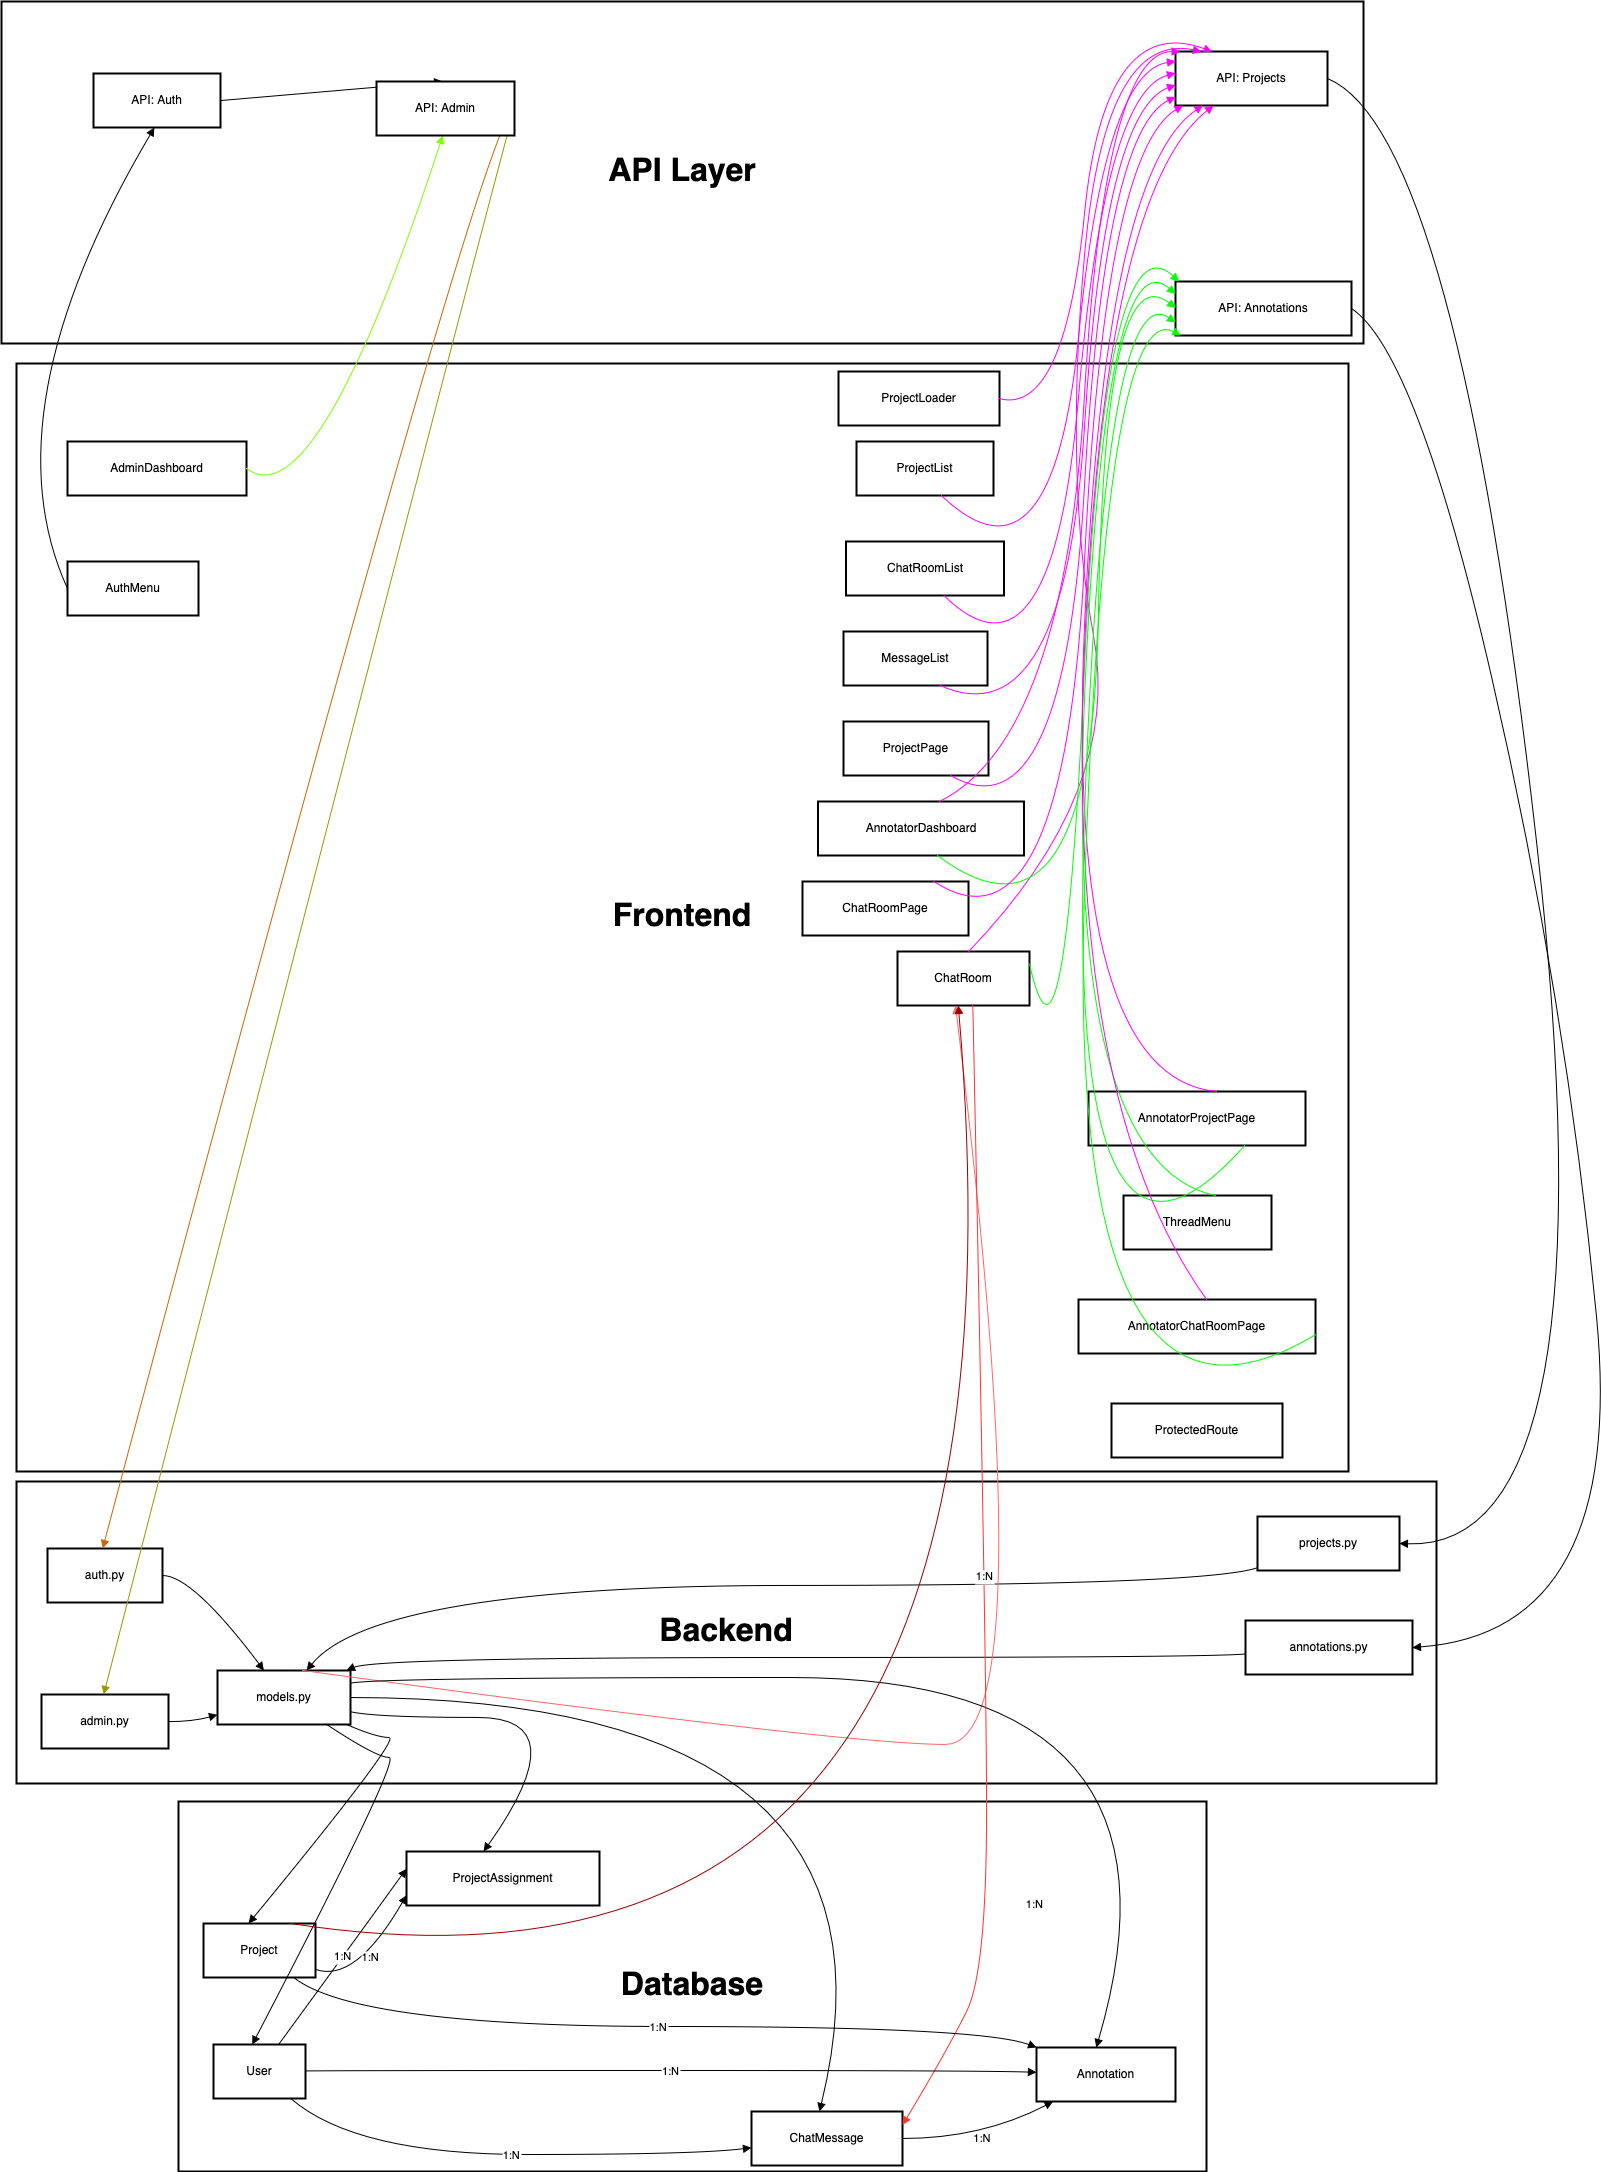
\includegraphics[width=0.95\textwidth,height=0.95\textheight,keepaspectratio]{images/2A-ERT-B.drawio.png}
    \caption{Modelo de Entidade-Relação do Sistema}
    \label{fig:modelo-er}
\end{figure}

\begin{landscape}
    \begin{figure}[p]
        \centering
        \makebox[\textwidth][c]{%
            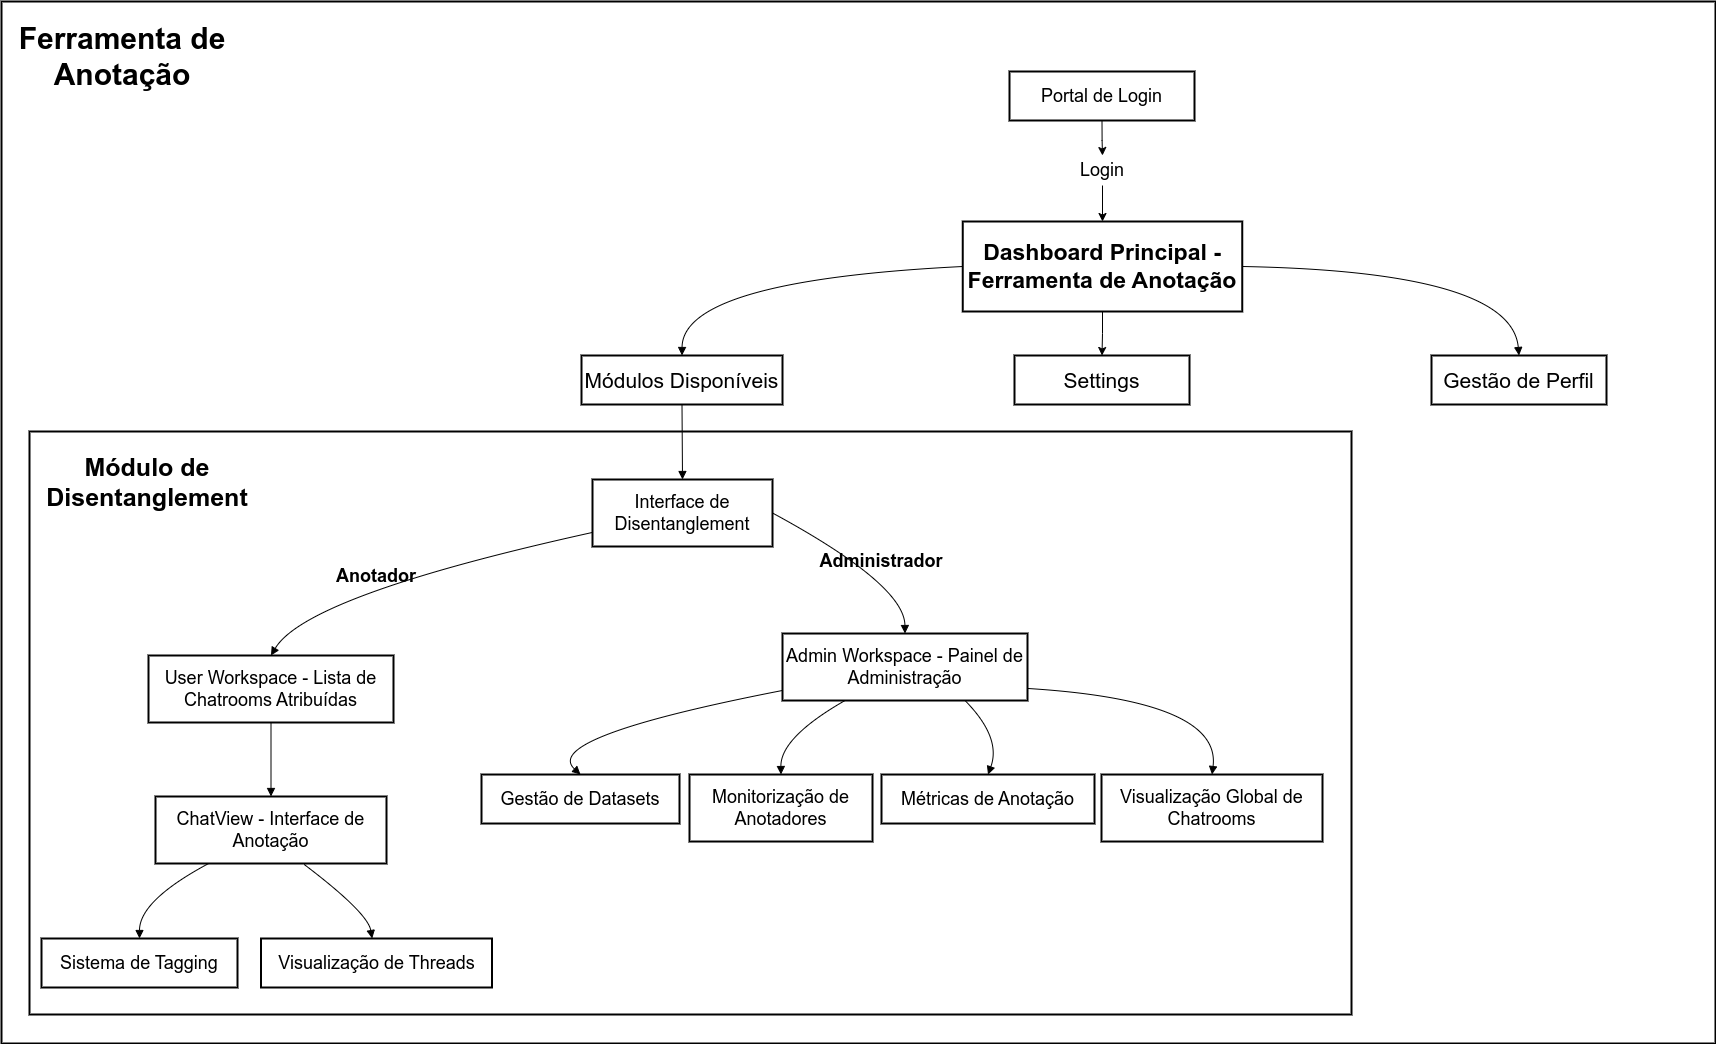
\includegraphics[width=0.8\paperheight, angle=0, keepaspectratio]{images/mapaDeNavegacaoSistema.drawio.png}
        }
        \caption{Mapa de Navegação do Sistema}
        \label{fig:mapa-navegacao}
    \end{figure}
\end{landscape}